\section{Plotting flashes}\seclab{DataSelect}

The raw lists of sources as generated by the impulsive and the TRI-D imagers of the LOFLI package are post-processed to produce images of the flash and supplementary data. The main objective is to select from the raw source files those sources that obey certain quality conditions (like the value of the chi-square for the impulsive imager) and fall within the designated time span and box in the atmosphere. It allows for tracking a leader and produce the distribution of the sources around the leader among other aspects.

The LINUX script \verb!DataSelect.sh! reads the input from DataSelect. The script \verb!DataSelect.bat! is for running under windows and uses the same input. Note that this script combines the functionality of the older scripts \verb!FlashImage! and \verb!InterfSrcSel!.

In its most basic form \verb!DataSelect.in! reads like

\begin{linenumbers}
\resetlinenumber
%\small
\footnotesize
%\scriptsize
%\tiny
\begin{verbatim}
&Parameters
datafile= "Srcs23-evenn", xyztBB= 15.75 +17.8  40 42.  3.5 5.5   1965 1990 ,  PlotName= "3b-N1"
&End
\end{verbatim}
\end{linenumbers}

A parameter block starts with \verb!&Parameters! and ends with \verb!&end! where the different parameters are separated by commas, and may spread over several lines. An input file can contain several parameter blocks. The most basic parameters are:
\begin{enumerate*}
\item \verb!datafile= "filename"!: specifying the name of the file that contains the list of raw sources. The quotation marks are essential and the extension is added automatically. The file should reside in the same folder where \verb!DataSelect! is run or otherwise the filename should contain the path. If the file in the folder has the extension \verb!.csv! is implies that the raw sources are generated by the impulsive imager.
\item \verb!xyztBB=!: followed by eight real values specifies the bounding box for the image. The expected order is minimum and maximum values for the x coordinate, followed by those for y, z, and time.
\item \verb!PlotName= "xxx"!: The names of all plots will be composed of three parts, first the name of the folder (impulsive imager, usually equal to the flash name) or the name of the datafile (TRI-D imager), followed by \verb!xxx!, and possibly followed by the name of a special purpose plot.
\end{enumerate*}
The complete list of possible parameters with a short explanation can be found in the \verb!DataSelect.out! file. Note that some options are specific for either impulsive imager data or for TRI-D data. We will discuss the different parameters as they are used for for various options.

\subsection{Flash image}

For generating a flash image the following parameters may also be important, beside the basic ones.

Specific options when using data from the impulsive imager, with their default value. All determine the quality conditions a source should obey to be plotted.
\begin{enumerate*}
\item \verb!RMS_ns= 4.0!: condition [$\sqrt(\chi^2) <$ \verb!RMS_ns!] in units [ns].
\item \verb!DelNEff= 25 ! (integer): condition when [\verb!DelNEff! $>0$] is [(\# of available antennas) - (\# number of used antennas)) $\leq$ \verb!DelNEff! ], where (\# of available antennas) is the number of antennas that have data for this source and (\# number of used antennas) is the number of antennas where the pulse from this source could be identified unambiguously.
\item \verb!LinCutH= 2.0!: condition: [$\sigma_h \times h <$ \verb!CutSigmaH! $\times$ \verb!LinCutH!] when [$h < $\verb!LinCutH!], unit [km], where $\sigma_h$ is the error in the altitude of a source as estimated by the impulsive imager at altitude $h$. The error in altitude is usually larger than those in Northing or Easting of the source. Additionally it is seen that this error grows with the altitude of the source which is the reason for the linear dependence. This quality indicator is particularly important when imaging ground strokes.
\item \verb!CutSigmaH= 17.0!: see above.
\item \verb!QualPlot= F !(logical): make a scatter plot of different quality indicators to investigate their correlations.
\end{enumerate*}

Specific options when using data from the TRI-D imager, with their default value:
\begin{enumerate*}
\item \verb!datafile= "xxx#+", "yyy" !: The \verb!"OutFileLabel="! from the different TRI-D runs for which the images have to be merged. This may also be just from a single run. The \verb!"#+"! in the name indicates that all files are collected that were generated by the TRI-D imager when it followed a leader path.
\item \verb!TimeBase=!: the default value is taken from the first file that is read.
\item \verb!SMPowCut= 500.0!: plot only those sources for which the intensity exceeds the specified limit.
\item \verb!StatNCut= F! (logical): keep only the ``\verb!FileStatN!" strongest sources of each TRI-D source file. This functions as a simple way to set a variable intensity threshold when a dart leader drastically changes its intensity as it propagates.
\item \verb!FileStatN= 5 !:Print the strength of the N$^{th}$ strongest source in the .out file. This was most useful for the estimate of the upper strength of positive leaders in Ref.~\cite{Scholten:2023PL}.
%\item[4] \verb!"! ZoomClip = .true."!: Only the points falling inside the plot boundary will be drawn.
\end{enumerate*}
When in \verb!datafile=! multiple source files are specified, these data will be merged and written to file. This file will have \verb!repack! in its name.


Some Generic options when using data from both imagers, with their default value:
\begin{enumerate*}
\item \verb!tCutl= 0.0!: lower end of block filter in time.
\item \verb!tCutu= 0.0!: upper end of block filter in time. This allows for blocking-out a single bright source that may even be outside the windowed area, but enters the picture through `side beams'.
\item \verb!BckgrFile= ""!: name of file that is displayed as a grey background plot.
\item \verb!ZoomBox= "NoBox" !:  name of the plot that zooms-in on a section of the present plot. This produces a box in the figure indicating the zoomed-in area. This option is used frequntly, see for example Ref.~\cite{Scholten:2021-HANL}.
\item \verb!AmplitudePlot=!  (Imp: =-1.00 ; TRI-D: =10.0): it sets the diameter of the largest symbols used in the plot. When zero or negative, a fixed size dot will be used for all points, independent of their intensity. Additionally the panel showing the intensity spectrum will not be shown.
\item \verb!NEhtBB=!: an alternative way to specify the bounding box using Northing, Easting, Altitude, and Time.
\end{enumerate*}


\begin{figure}[th]
\centering{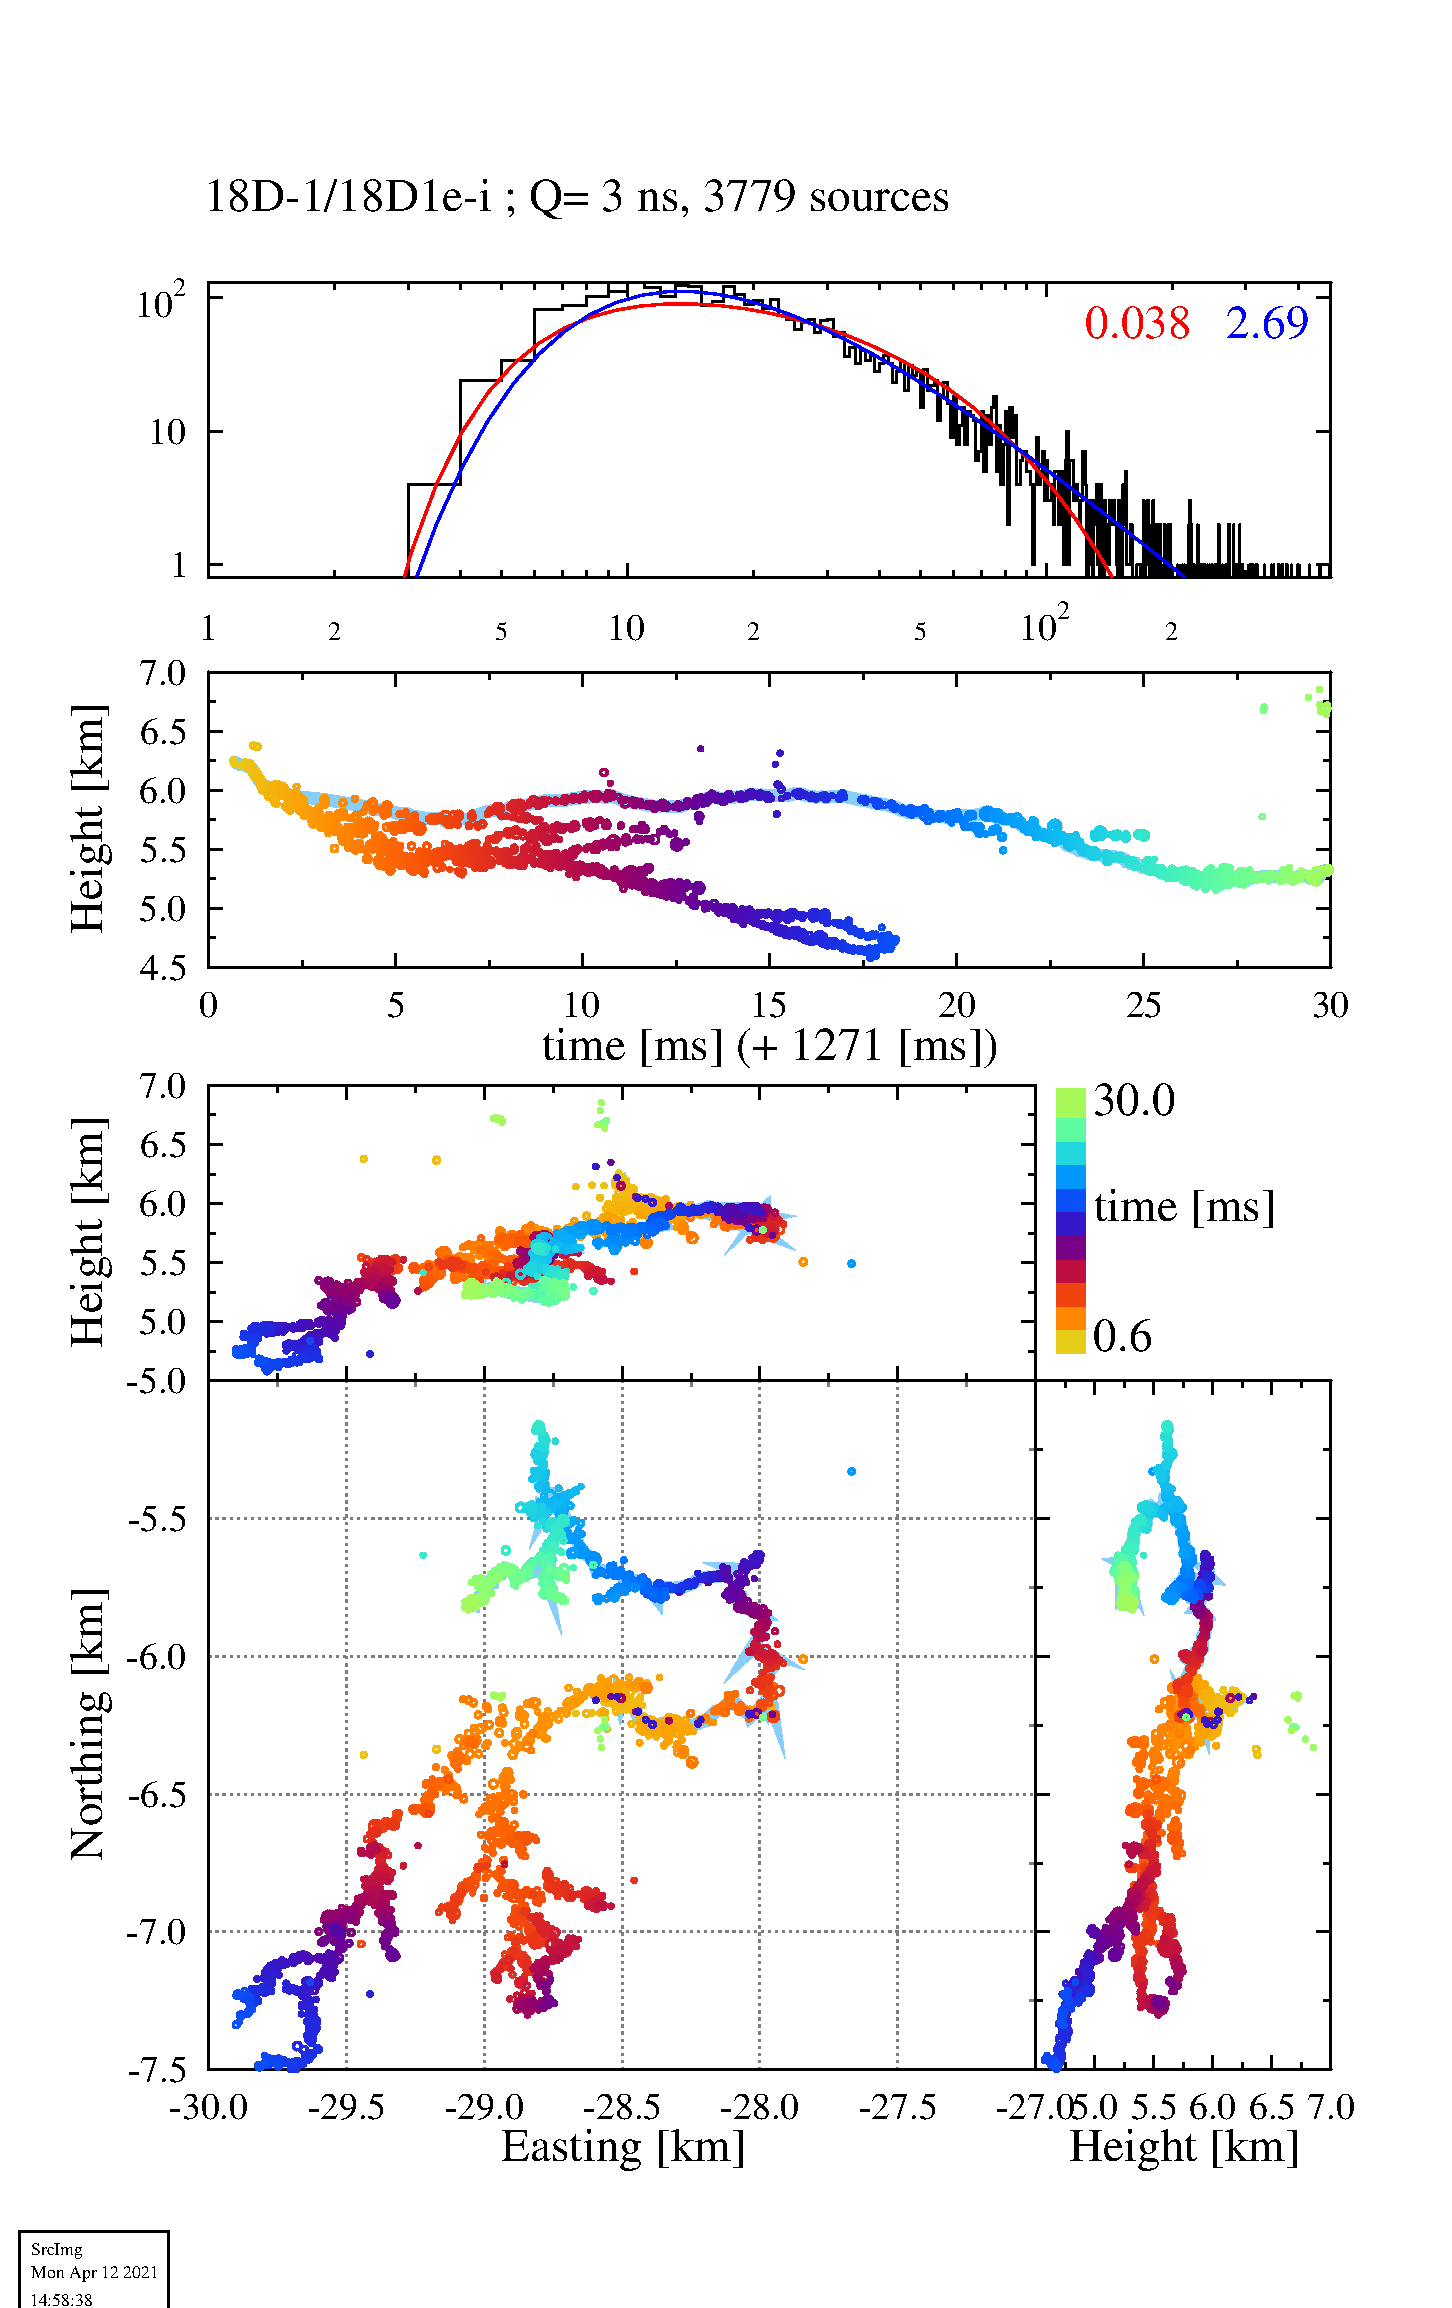
\includegraphics[width=0.49\textwidth]{Figs/Imp_18D1e-i} }
\centering{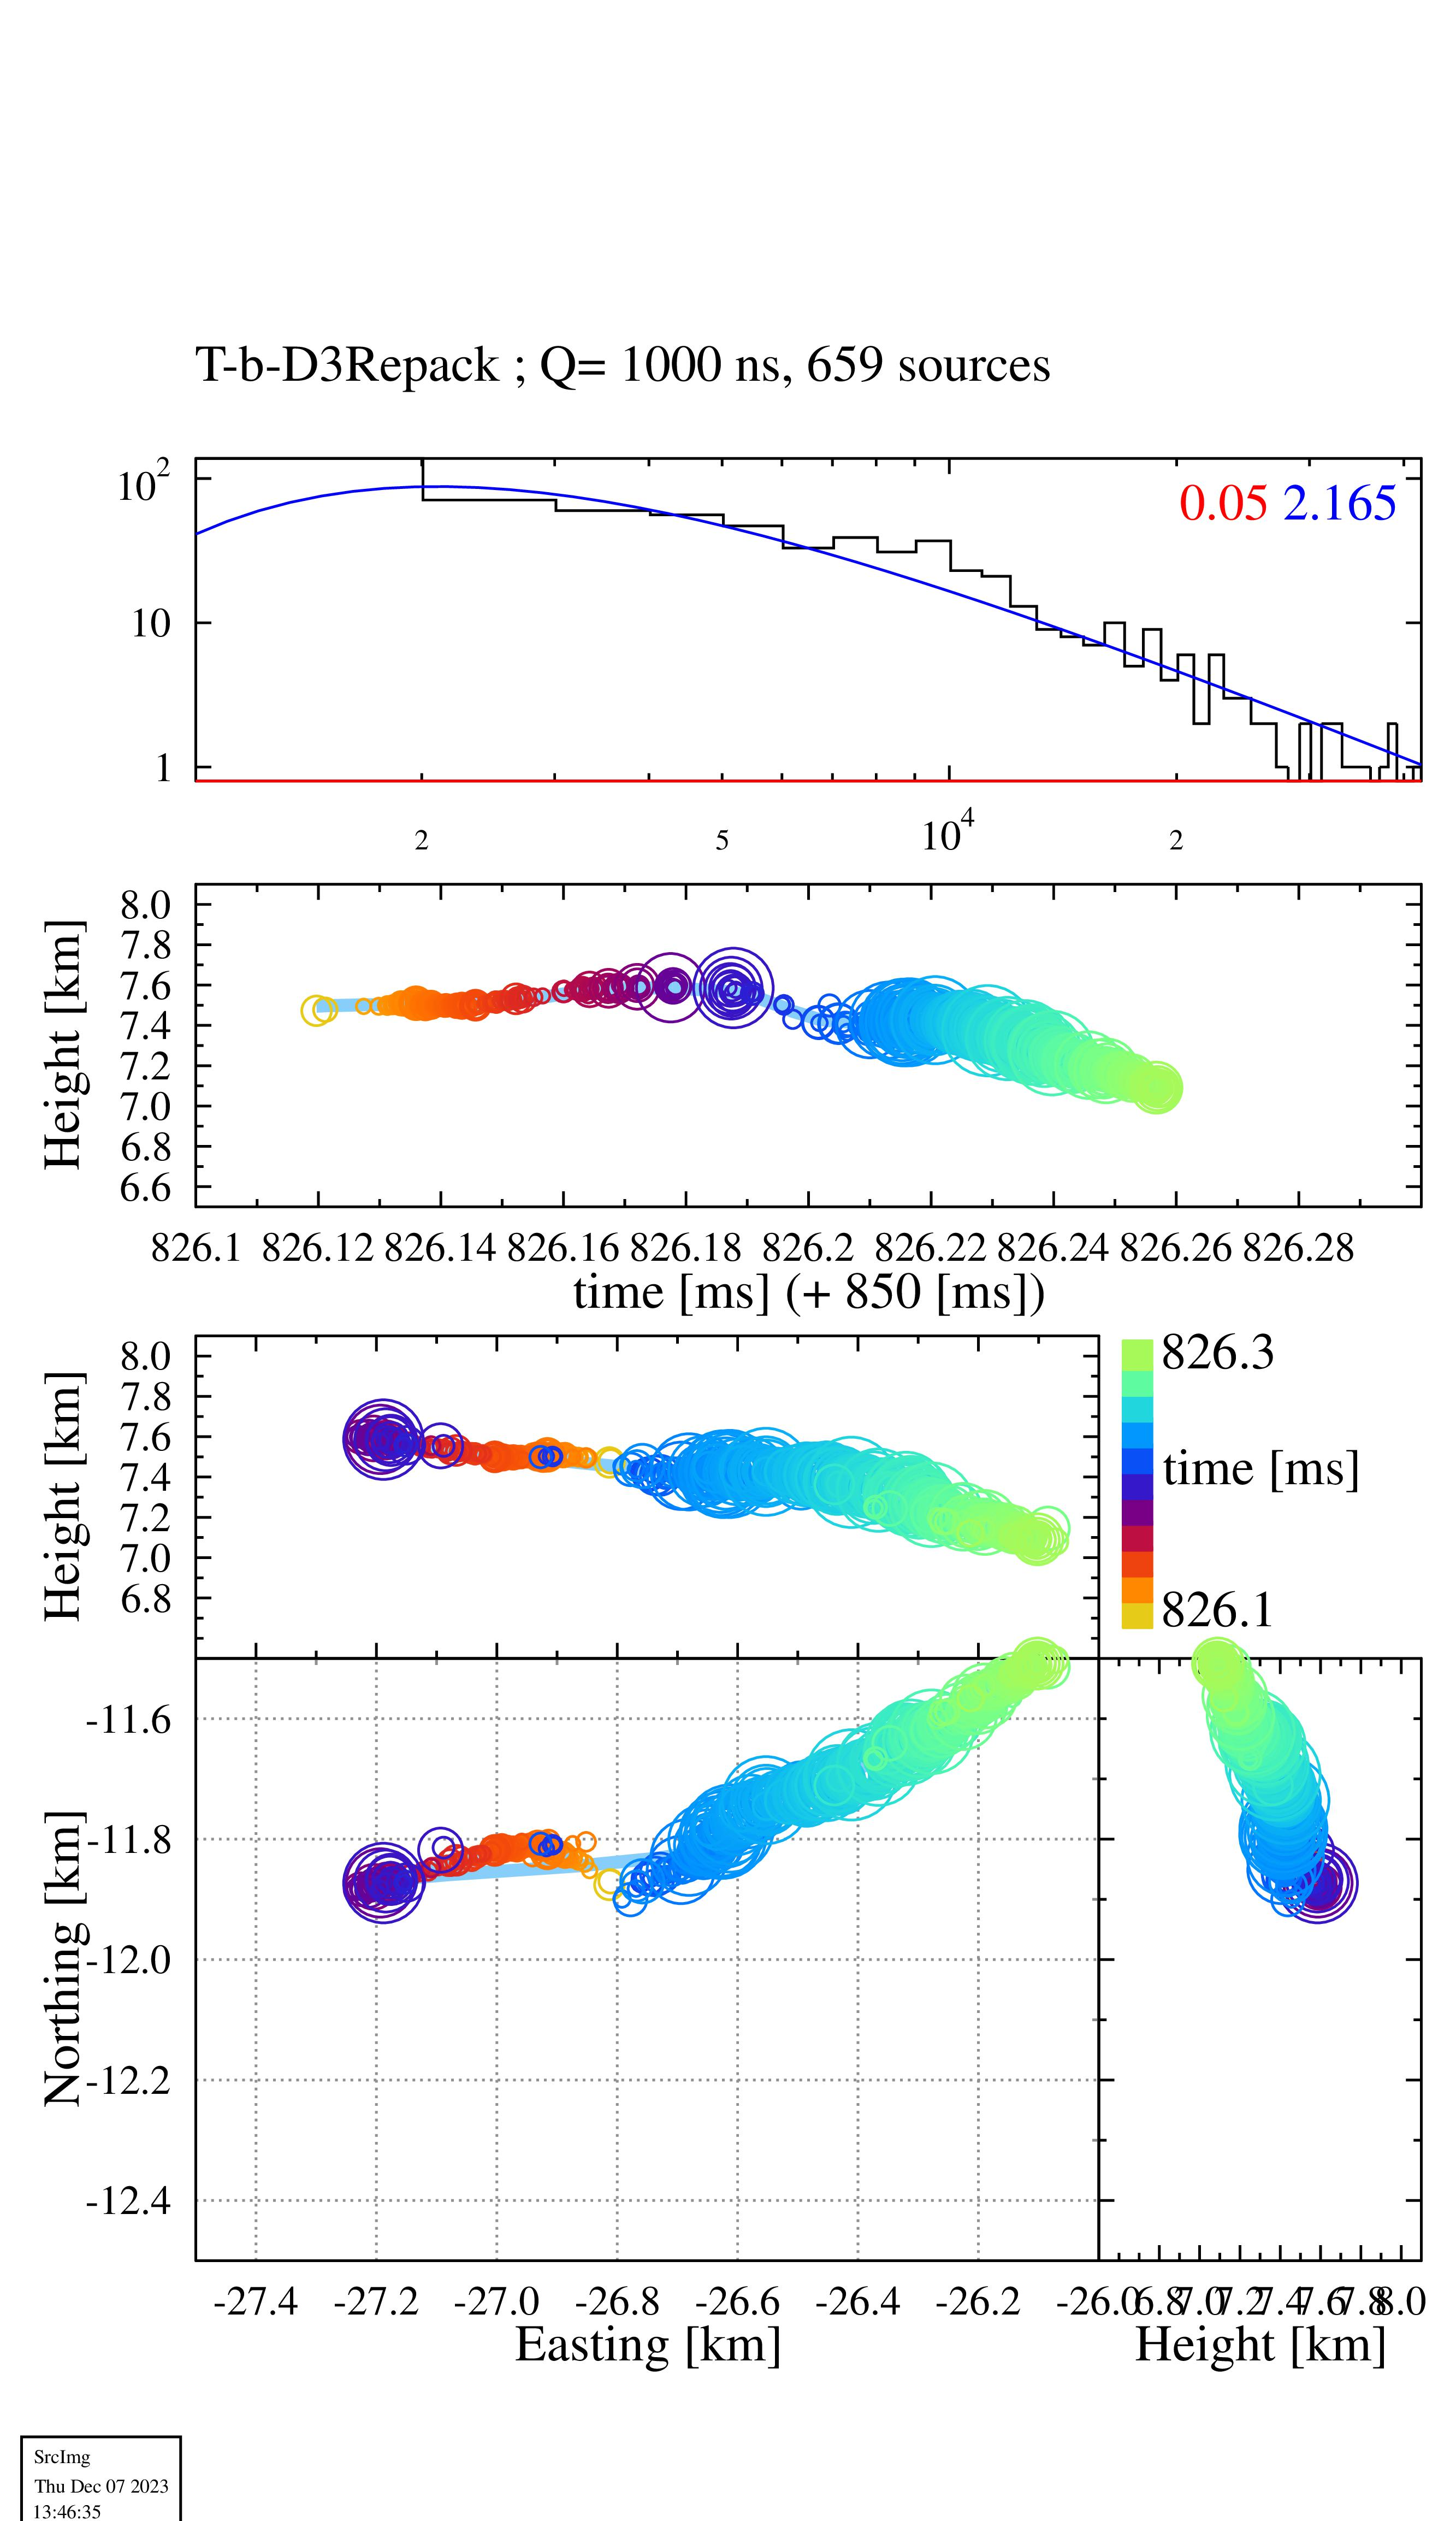
\includegraphics[width=0.49\textwidth]{Figs/T-b-D3Repack} }
%\centering{\includegraphics[ bb=1.0cm 2.4cm 24.5cm 25.7cm,clip, width=0.49\textwidth]{../Figs/SE20A7-NPMx_1HIntfSpecSel} }
	\caption{Typical image for the Impulsive Imager (left) and the TRI-D imager (right) as created by running ``DataSelect.bat". Light blue band is the reconstructed track (starting from the latest point and tracing back). Top panel give pulse power statistics where the modified exponential is plotted in red and the modified power law plotted in blue.}	 \figlab{ImpulsiveImg}
\end{figure}


The produced .dat files are plain text files and contain some header lines with some general information followed by the specific data of the sources. The files have a format that is suitable for the plotting script \verb!"SourcesPlot.gle"!.


Two gle-scripts \verb#'%UtilDir%Intensity.gle'# and \verb#'%UtilDir%SourcesPlot.gle'# make the following plots.

\begin{figure}[h]
\setlength{\unitlength}{.48\textwidth} % .43\textwidth}
   \subfloat[Figure `IntfSpecSel']{ 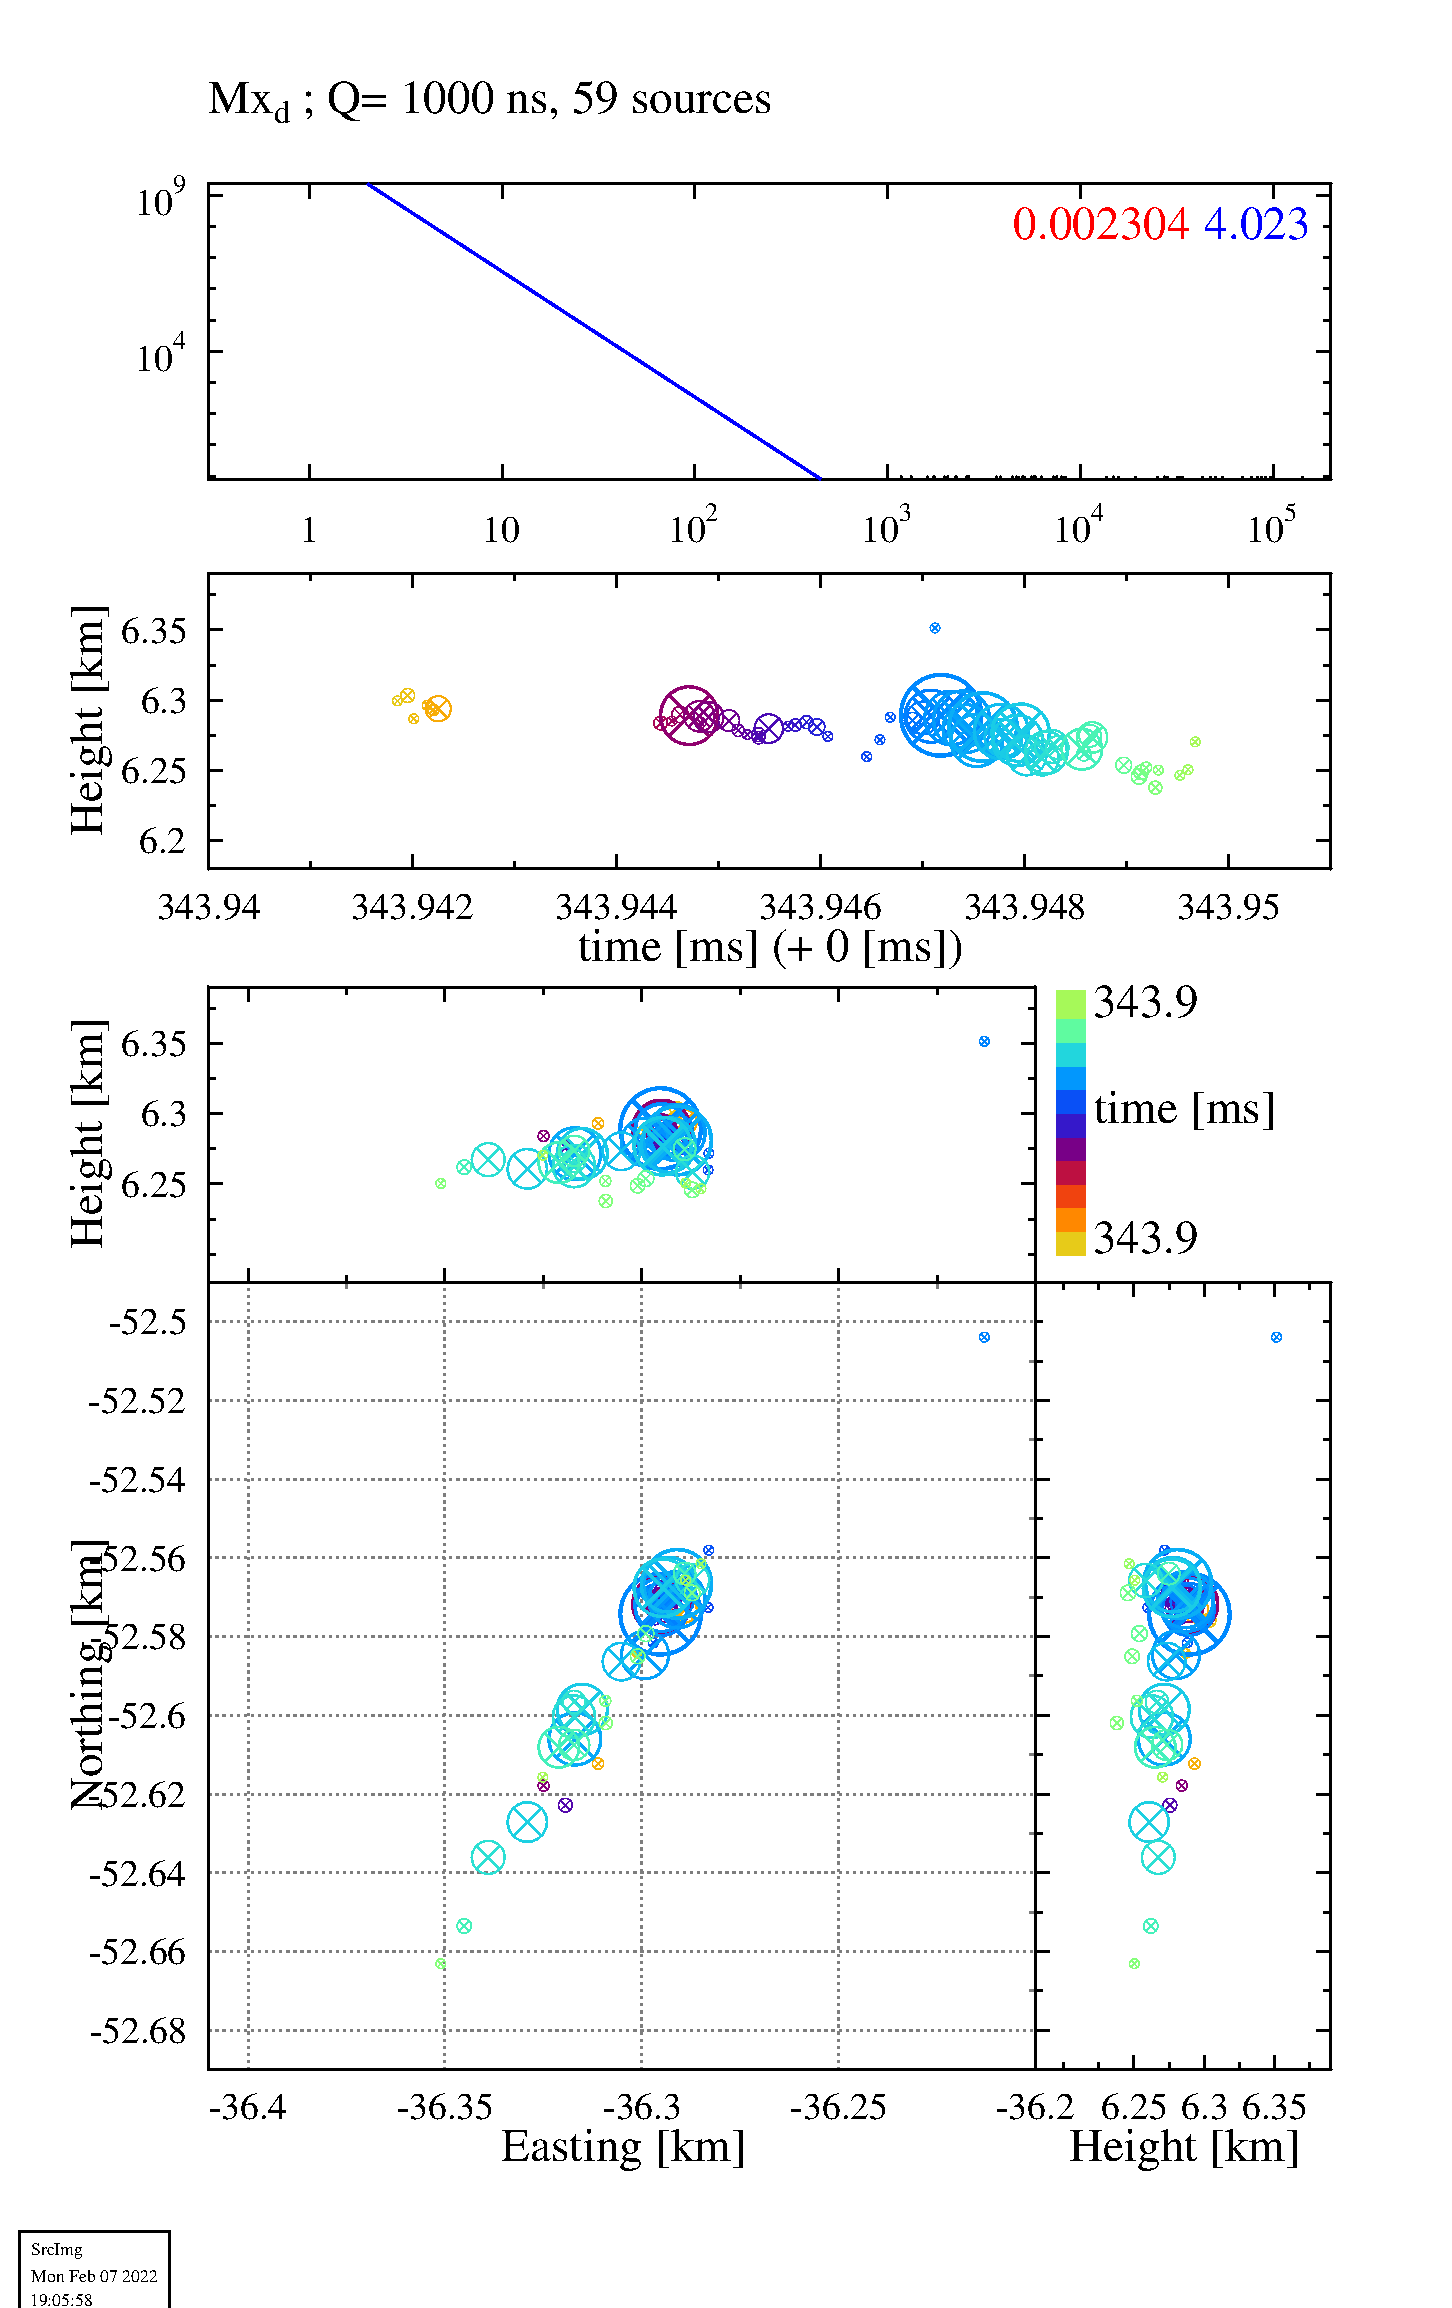
\includegraphics[width=\unitlength]{Figs/Mx_dIntfSpecSel}  \figlab{InterfSrc-Spec}}
   \subfloat[Figure `AmplFit']{ 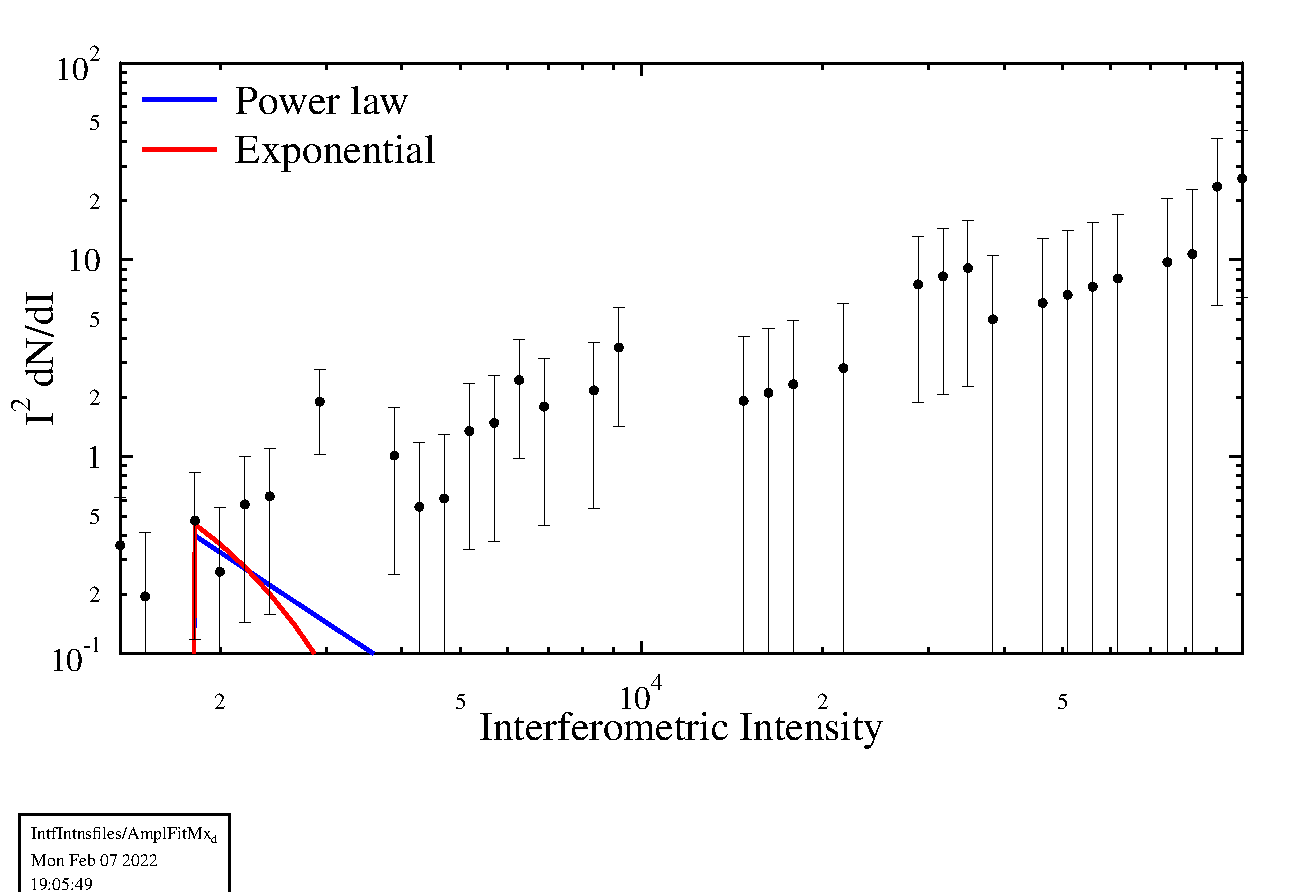
\includegraphics[width=\unitlength]{Figs/Mx_dAmplFit}  \figlab{InterfSrc-Ampl}}
	\caption{Top panel in \figref{InterfSrc-Spec} shows the intensity distribution of the sources and two fits (that obviously do not resemble the data for this case). The lower panels the usual way of plotting the sources where the size of the circles reflects the intensity.
\figref{InterfSrc-Ampl} displays an attempt to fit the pulse-strength distribution.}	 \figlab{InterfSrc}
\end{figure}

Obviously more writing needs be done, but this is it for the time being.

\subsection{Track finding}

Produces, among other aspects of a leader, the velocity distribution along the leader track as used in Ref.~\cite{Scholten:2021-RNL}

Some Generic options when using data from both imagers, with their default value:
\begin{enumerate*}
\item \verb!NLongTracksMax= 0 !: Maximum number of tracks to include in plot
\item \verb!MaxTrackDist= !: Max. distance between sources to include on a track.
\item \verb!Wtr=!: Weight of newest source for track centroid.
\item \verb!Aweight= 0.0!: Importance of intensity in weight of newest source for track centroid.
\item \verb!TimeWin=!: [ms]. Width of gaussian in time to weigh the sources for mean track position.
\item \verb!PreDefTrackFile= ""!: Label of file that contains a track to be included.
\item \verb!dt_MTL=!: [ms]. Time-step for constructing tracks.
\item \verb!HeightFact= 0.0!: Relative height scale for calculating distances.
\item \verb!SrcDensTimeResol=!: [ms]. Source Density Time Resolution.
\end{enumerate*}


\begin{figure}[th]
\centering{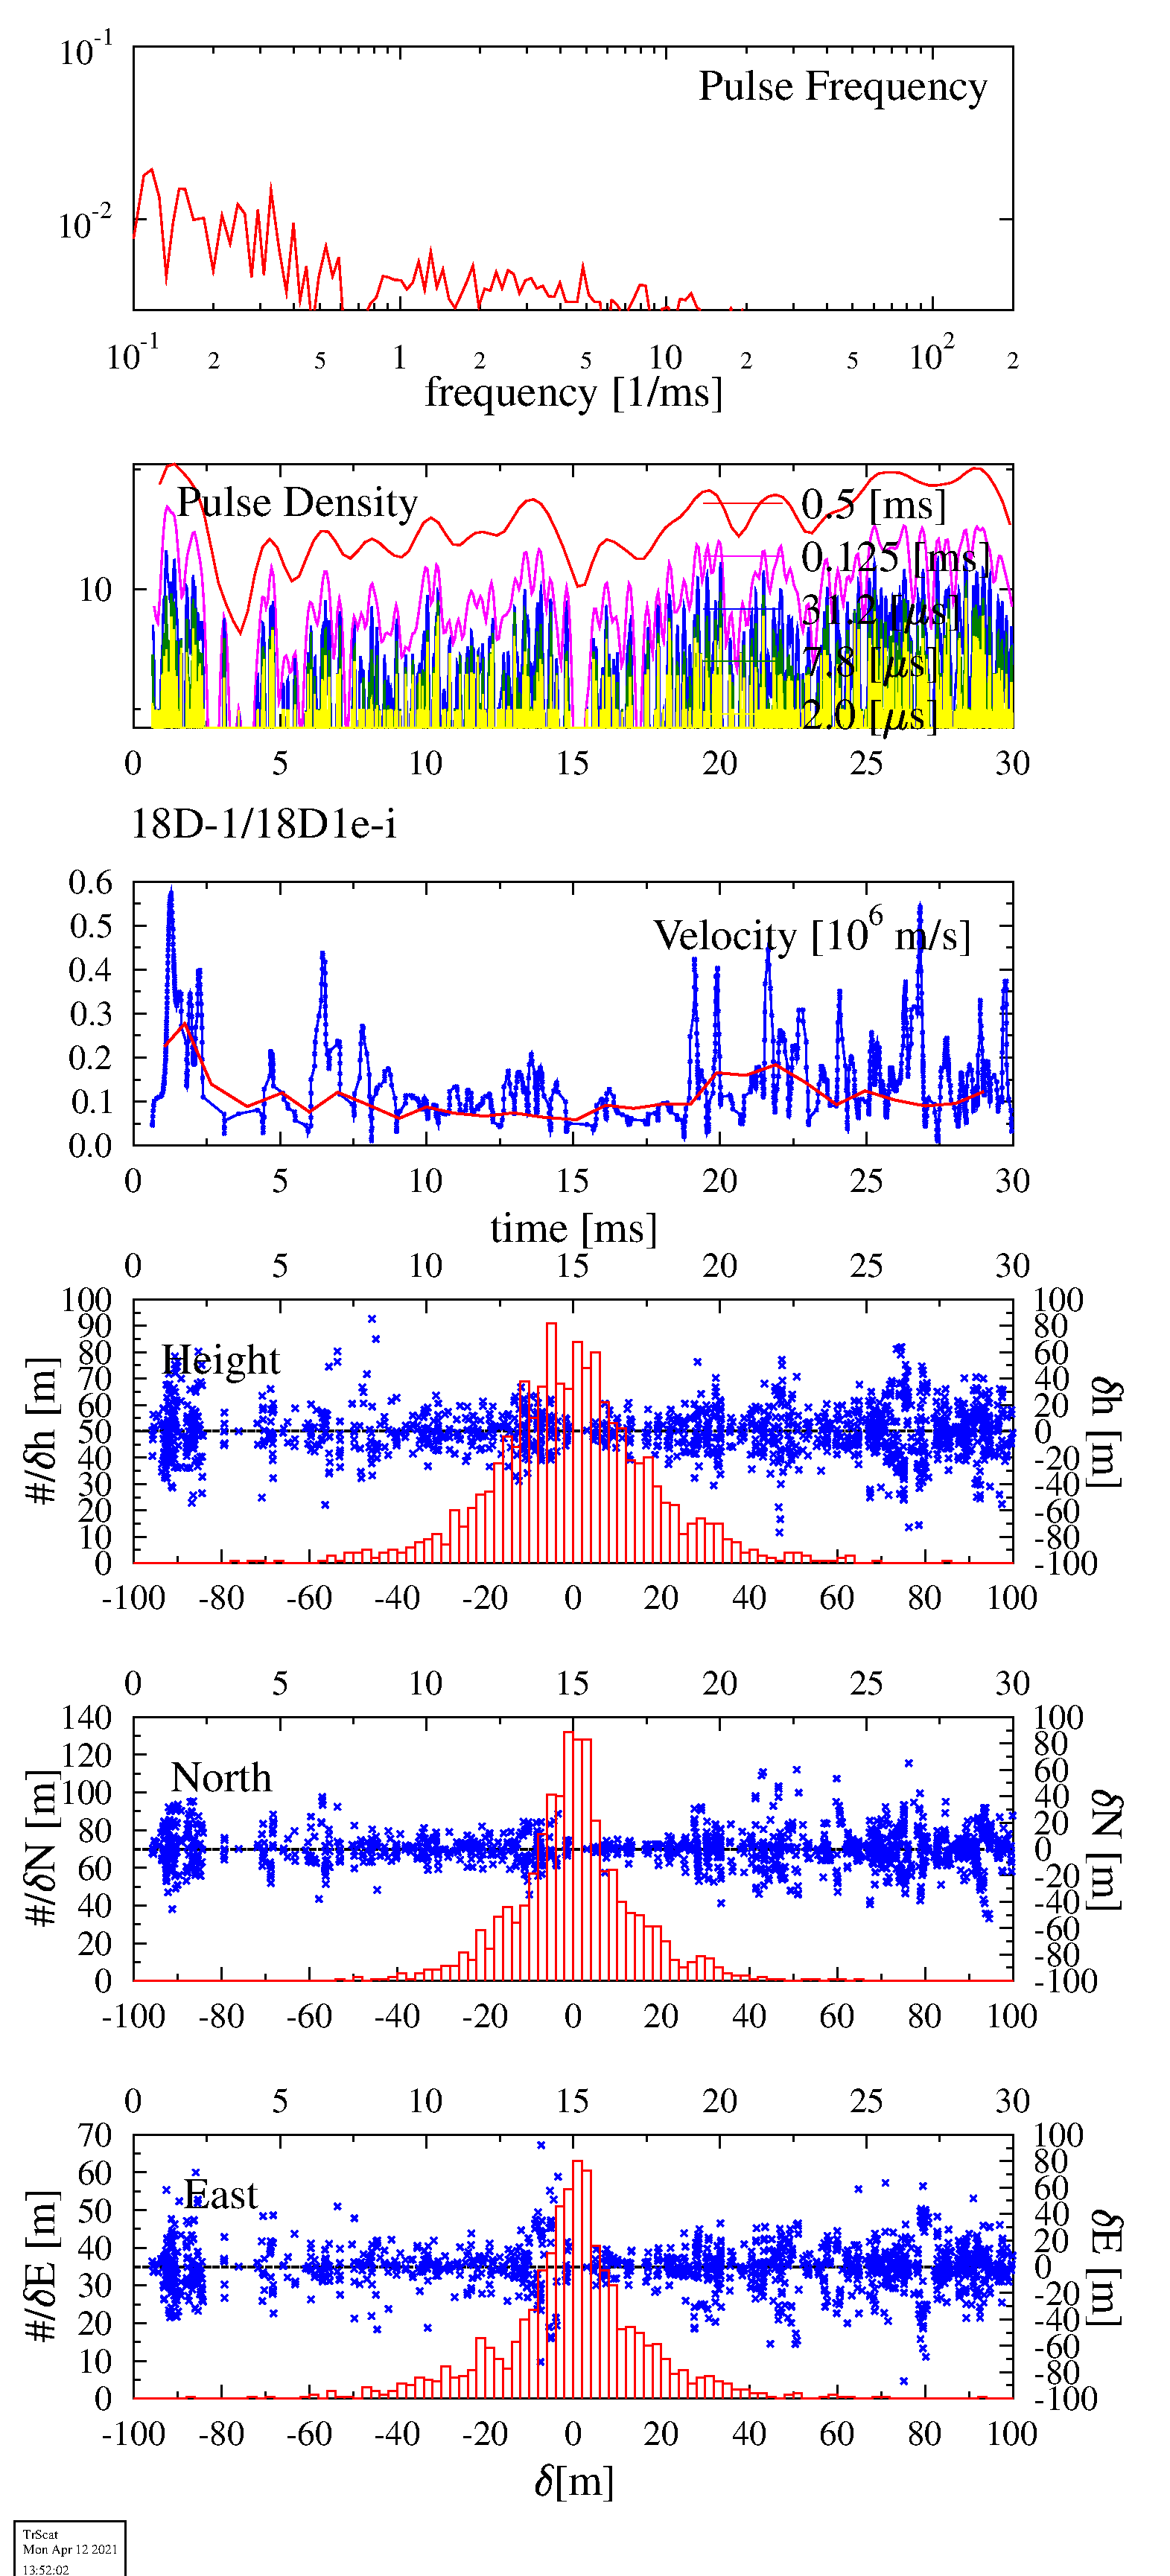
\includegraphics[ width=0.49\textwidth]{Figs/TrSc_18D1e-i} }
%\centering{\includegraphics[ bb=1.0cm 2.4cm 24.5cm 25.7cm,clip, width=0.49\textwidth]{../Figs/SE20A7-NPMx_1HIntfSpecSel} }
	\caption{Typical image for the Impulsive Imager when showing the statistics along a track.}	 \figlab{ImpulsiveTrack}
\end{figure}

If the 7th number on the second line in the input, ``FlashImage.in", is positive, a graph like \figref{ImpulsiveTrack} is made for each track. The second panel from the top shows the pulse density along the flash as function of time for various width of a gaussian smoothing function. The top panel shows the fourier decomposition of this plot. The third from the top gives the velocity along the track. The blue line for each source along the track, the red line for an average leader-tip location. The bottom three panels show the spread of the sources in the three directions from the propagating tip of the leader, in blue as a scatter plot v.s.\ time of the source (top and right scales), in red as a histogram (bottom and left scales).

For TRI-D based images a Principal Component analysis is performed on the direction of the polarization vector for each slice and a plot is make.

\subsection{Power spectrum}
Produces a power-law fit to source intensities, much like what was used in Ref.~\cite{Machado:2021, Scholten:2021-INL}

Some Generic options when using data from both imagers, with their default value:
\begin{enumerate*}
\item \verb! MaxAmplFitPercent= 0.1 !: Max amplitude fitted with modifies power law. (TRI-D only?)
\end{enumerate*}

The result is displayed in \figref{ImpulsiveImg} for the image of the flash for the selected area. The normalized pulse powers distributions $N(I)$ are fitted with a modified exponential,
\begin{equation}
N(I)= {\cal N}_e \,e^{-\alpha_e\,I-\gamma_e/I^2}\;, \eqlab{PowLaw}
\end{equation}
as well as with a modified powerlaw,
T\begin{equation}
N(I)= {\cal N} \,I^{-\alpha}  \,e^{-\gamma/I}\;, \eqlab{PowLaw}
\end{equation}
where $I$ is expressed in units of [GB]. The last factor, dependent on $\gamma$, suppresses the distribution at small amplitudes to good agreement with the data. The values for the fitted values for the normalization ${\cal N}$, the power $\alpha$, and the small-intensity suppression factor $\gamma$ are given in the output file (with extension .out).

The out file %\verb#'IntfrSrcSel.out'# looks like

\begin{linenumbers}
\tiny
\resetlinenumber
\begin{verbatim}
 ======================  Mx_d
 After file:files/IntfSpecPowMx_d.dat, SourcTotNr=          59
 Time span data=   343.94184999999999        343.94967000000003
Amplitudes (#=      59), max@ 198243.0, 5-pctile@********, 10-pctile@87401.70
Amplitude with   0.001pctile as included in fit @********
 $b *exp(-a*A-c/A^2); \chi^2=$  0.98,with  a,b,c=  0.0023 0.903E-05   0.00    ; nrm=  0.805E+05
 $b *A^-a *exp(-c/A); \chi^2=$  0.97,with  a,b,c=   4.023 0.156E+07   0.00    ; nrm=  0.805E+05
 $b *exp(-a*A-c/A^2); \chi^2=$  0.98,with  a,b,c= 0.2304E-020.9031E-05   0.00    ; nrm=   6.10      0.805E+05
 $b *A^-a *exp(-c/A); \chi^2=$  0.97,with  a,b,c=  4.023    0.1562E+07   0.00    ; nrm=   7.04      0.805E+05
 number of sources in plots:          59   1000.0000000000000      Mx_dIntfSpecSel
 ======================  End input
\end{verbatim}
\end{linenumbers}

Showing the number of points that fall within the plot boundary. A fit is made to the power spectrum for different functional dependencies and the resulting parameters are specified.

\subsection{Space-time correlation}

Produces the space-time correlation plots as used in Ref.~\cite{Wang:2023}

The calculation of TD correlators requires positive values for "Corr\_dD" and "Corr\_Dnr"
\begin{enumerate*}
\item \verb!Corr_dD !: Distance step size for time-distance correlator.
\item \verb!Corr_Dnr!: max. number of distance bins for time-distance correlator.
\item \verb!Corr_dtau=!: Time step size for time-distance correlator.
\end{enumerate*}


\clearpage 